\documentclass{beamer}

\usepackage[utf8]{inputenc}
\usepackage[T1]{fontenc}
\usepackage{multicol}
\usepackage{amsthm}
\usepackage{amsmath}
\usepackage{amssymb}
\usepackage{mathtools}
\usepackage{dsfont}
\usepackage{bbm}
\usepackage{xparse}
\usepackage{physics}
\usepackage{empheq}
\usepackage{url}
\usepackage{hyperref}
\usepackage{tikz}
\usetikzlibrary{quotes,angles,calc}
\usepackage{rotating}
\usepackage{graphicx}
\usepackage[linesnumbered,ruled,vlined]{algorithm2e}
\SetKwInput{KwInput}{Input}                % Set the Input
\SetKwInput{KwOutput}{Output}              % set the Output

\theoremstyle{definition}
\newtheorem{theo}{Theorem}[section]
\newtheorem{lem}[theo]{Lemma}
\newtheorem{cor}[theo]{Corollary}
\newtheorem{prop}[theo]{Property}
\newtheorem{defi}[theo]{Definition}

\theoremstyle{remark}
\newtheorem*{rk}{Remark}

\DeclareMathOperator{\maxi}{\text{maximize}}
\DeclareMathOperator{\mini}{\text{minimize}}
\DeclareMathOperator{\st}{\text{subject to}}
\DeclarePairedDelimiter\ceil{\lceil}{\rceil}
\DeclarePairedDelimiter\floor{\lfloor}{\rfloor}
\DeclarePairedDelimiterX\set[1]\lbrace\rbrace{\def\given{\;\delimsize\vert\;}#1}

\colorlet{darkgreen}{green!40!black}

\usetheme{Dresden}
\usecolortheme{lily}
\newcommand*\oldmacro{}%
\let\oldmacro\insertshorttitle%
\renewcommand*\insertshorttitle{%
  \oldmacro\hfill%
  \insertframenumber\,/\,\inserttotalframenumber}


\title{Algorithmic aspects of Optimal Channel Coding:\\ A geometric point of view}
\author{Paul Fermé}
\institute{LIP - ENS de Lyon}
\date{20/04/20}

%\AtBeginSection[]
%{
%  \begin{frame}<beamer>
%    \frametitle{Contents}
%    \tableofcontents[currentsection]
%  \end{frame}
%}

%%%%%%%%%%%%%%%%%%%%%%%%%%%%%%%%%%%%%%%%%%
\begin{document}
%%%%%%%%%%%%%%%%%%%%%%%%%%%%%%%%%%%%%%%%%%

\begin{frame}
  \titlepage
\end{frame}

%%%%%

\begin{frame}{Introduction}
  \begin{itemize}
  \item How much classical information can we send through quantum channels?
\item Shannon and Holevo's \emph{channel capacity}: average number of bits per channel we can faithfully transmit in the limit of taking $n$ channel copies.

  \pause
  \bigskip
  
  \item \underline{Our setting:} what is the \emph{best} strategy (maximizing the probability of success) of sending $k$ equiprobable messages through \emph{one} channel.
  \item How efficiently can we compute a \emph{good} strategy?
  \end{itemize}
\end{frame}

\begin{frame}{Contents}
  \tableofcontents
\end{frame}


%%%%%%%%%%%%%%%%%%%%%%%%%%%%%%%%%%%%%%%%%%
\section{Channel Coding Function}
%%%%%%%%%%%%%%%%%%%%%%%%%%%%%%%%%%%%%%%%%%
\begin{frame}{Channel Coding Function}
  \begin{defi}[Channel Coding Function]
    $W = \set{W_x}_{x \in X}$ a classical-quantum channel, ie. a finite set of quantum states. $S \subseteq X$ a code for $\abs{S}$ messages, best POVM gives

    \only<1>{
  \begin{equation}
    \begin{aligned}
      & g_W(S) :=&& \underset{\Lambda}{\maxi} &&\frac{1}{\abs{S}}\underset{x \in S}{\sum} \Tr(\Lambda_x W_x) \\
      &&& \st && \underset{x \in S}{\sum} \Lambda_x = \mathbbm{1}\\
      &&&&& \Lambda_x \succcurlyeq 0, \forall x \in S
    \end{aligned}
    \end{equation}}
    
    \pause
    
  \begin{equation}
    \begin{aligned}
      & \color{red} f_W(S) :=&& \underset{\Lambda}{\maxi} && \color{red} \underset{x \in S}{\sum} \Tr(\Lambda_x W_x) \\
      &&& \st && \underset{x \in S}{\sum} \Lambda_x = \mathbbm{1}\\
      &&&&& \Lambda_x \succcurlyeq 0, \forall x \in S
    \end{aligned}
  \end{equation}
  \end{defi}

 The probability of success of the best strategy is given by:
  \[S(W,k) := \textcolor{red}{\frac{1}{k}} \underset{S \subseteq X, \abs{S} \leq k}{\max} \textcolor{red}{f_W(S)}\]
  
\end{frame}

\begin{frame}{First examples on the Bloch sphere}
  \begin{columns}
    \begin{column}{6cm}
      \begin{center}
        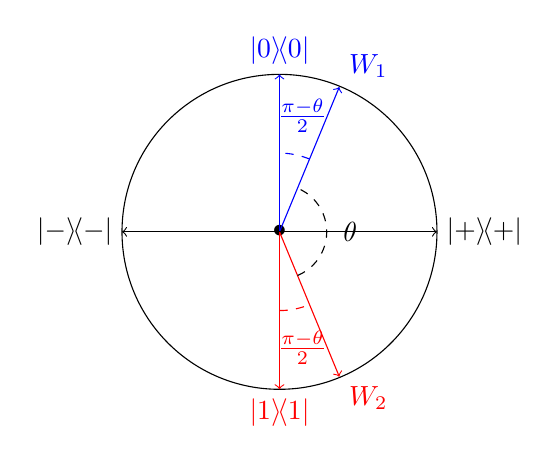
\begin{tikzpicture}
          \draw (0,0) coordinate (C) node {$\bullet$} circle (2);
          \draw[->, blue] (0,0) -- (0,2) coordinate (k0) node[above] {$\dyad{0}$};
          \draw[->,blue] (0,0) -- (0.76,1.84) coordinate (W1) node[above right] {$W_1$};
          \draw[->, red] (0,0) -- (0.76,-1.84) coordinate (W2) node[below right] {$W_2$};
          \draw[->,red] (0,0) -- (0,-2) coordinate (k1) node[below] {$\dyad{1}$};
          \draw[->] (0,0) -- (2,0) node[right] {$\dyad{+}$};
          \draw[->] (0,0) -- (-2,0) node[left] {$\dyad{-}$};
          \draw[dashed] pic["$\theta$", draw=black, angle eccentricity=1.5, angle radius=0.6cm] {angle=W2--C--W1};
          \draw[dashed,blue] pic["$\frac{\pi - \theta}{2}$", draw=blue, angle eccentricity=1.5, angle radius=1cm] {angle=W1--C--k0};
          \draw[dashed,red] pic["$\frac{\pi - \theta}{2}$", draw=red, angle eccentricity=1.5, angle radius=1cm] {angle=k1--C--W2};
        \end{tikzpicture}
      \end{center}
    \end{column}
    \begin{column}{5cm}
      Any $S$ such that $\abs{S} = 1$\\
      Best POVM = $\mathbbm{1}$\\
      $f(S) = 1, S(W,1) = 1$

      \bigskip
      \pause

      $W = \set{W_1,W_2}$ pure states.\\
      We take $S = \set{1,2}$.\\
      Best POVM is $\set{\dyad{0},\dyad{1}}$:\\
      \begin{equation*}
        \begin{aligned}
          f_W(S) & = 2\cos^2\Big(\frac{\pi-\theta}{4}\Big)\\
          & = 1 + \sin{\frac{\theta}{2}}\\
          S(W,2) & = \frac{1 + \sin{\frac{\theta}{2}}}{2}
        \end{aligned}
      \end{equation*}
    \end{column}
    \end{columns}

\end{frame}

\begin{frame}{Dual point of view}
  Finding a measurement is hard, we look at the (SDP) dual POV:
  \begin{prop}[Strong Duality]
  \begin{equation}
    \begin{aligned}
      &f_W(S) =&& \underset{\rho}{\mini} && \tr(\rho) \\
      &&& \st && \rho \succcurlyeq W_x, \forall x \in S
      \end{aligned}
  \end{equation}
  \end{prop}

  \pause

  \begin{prop}[\cite{Bae13}]
    The optimal matrix $\rho$ is unique, whereas the optimal POVM $\Lambda$ isn't (proved via KKT conditions: primal and dual constraints mixed).
  \end{prop}

  \begin{rk}
    The problem of computing one image of $f_W$ is known as \emph{minimum-error quantum state discrimination}.
  \end{rk}
\end{frame}

%%%%%%%%%%%%%%%%%%%%%%%%%%%%%%%%%%%%%%%%%%
\section{Geometric Point of View}
%%%%%%%%%%%%%%%%%%%%%%%%%%%%%%%%%%%%%%%%%%
\begin{frame}{Geometric point of view}
  \begin{defi}[Penumbra (inspired by \cite{BBPWW07})]
    $P(M) := \set{N \in \mathcal{H}_d \text{ s.t. } N \preccurlyeq M}$. It is a proper affine cone.
  \end{defi}

  \pause 
  \begin{prop}
    $Q_d := \mathcal{D}_d-\mathbbm{1}_d$ centered set of states.

    \bigskip
    
    Then $\mathcal{D}(m,r) := m-rQ_d$ with $m \in T_1  := \set{\tr(M)=1} \cap \mathcal{H}_d$ is the base of $P(m + r\mathbbm{1}_d)$ included in $T_1$.

    \bigskip
    \pause
    In particular for $W \in \mathcal{D}_d$ and any $M$ with $\tr(M) \geq 1$:
    \[W \in \mathcal{D}(m,r) \iff m + r\mathbbm{1}_d \succcurlyeq W\]
    \[M \succcurlyeq W \iff W \in \mathcal{D}(M - r_M\mathbbm{1}_d,r_M) \text{ where } r_M := \tr(M)-1 \]
    \label{propbase}
  \end{prop}
\end{frame}

\begin{frame}{Drawing}
  \begin{center}
    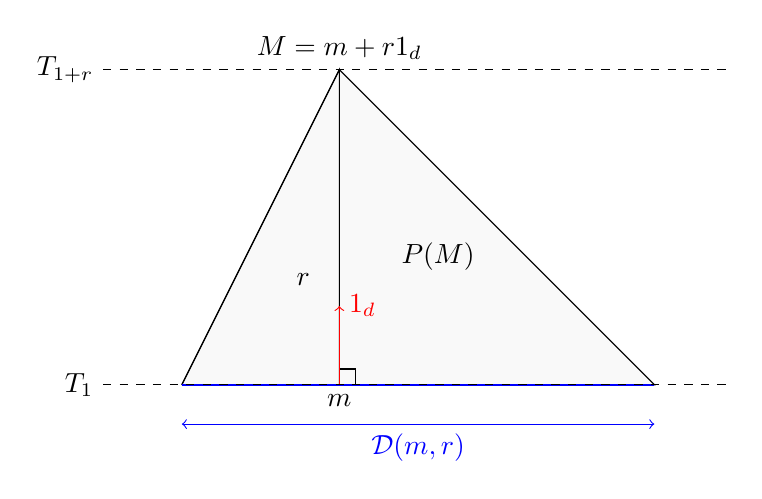
\begin{tikzpicture}
      \draw (0,0) coordinate (m') -- (6,0) coordinate (m'') -- (2,4) coordinate (M)  node [above] {$M = m + r\mathbbm{1}_d$};
      \draw[draw,fill=gray!05] (m')--(M)--(m'');
      \draw (m') -- (M) -- (2,0) coordinate (m) node[below] {$m$};
      \draw ($($(m)+(0,0.2)$)$) -- ($($(m)+(0.2,0.2)$)$) -- ($($(m)+(0.2,0)$)$);
      \draw ($1/3*($(m)+(M)$)$) node[right] {$r$};
      \draw ($1/3*($(m')+(M)+(m'')$)$) node[above right] {$P(M)$};
      \draw[<->,blue] ($($(m')-(0,0.5)$)$) coordinate (c) -- ($($(m'')-(0,0.5)$)$) coordinate (d);
      \draw[blue] ($1/2*($(c)+(d)$)$) node[below] {$\mathcal{D}(m,r)$};
      \draw[thick,blue] (m') -- (m'');
      \draw[red,->] (m) -- ($($(m)+(0,1)$)$) node[right] {$\mathbbm{1}_d$};
      \draw[dashed] ($($(m')-(1,0)$)$)  node[left] {$T_1$}  -- ($($(m'')+(1,0)$)$);
      \draw[dashed] ($($(M)-(3,0)$)$)  node[left] {$T_{1 + r}$}  -- ($($(M)+(5,0)$)$);
    \end{tikzpicture}
  \end{center}
\end{frame}

\begin{frame}{Equivalent geometric formulation}
  Let $W$ a finite set of points in $\mathcal{D}_d$, and $S$ a subset of its indices:
  \begin{itemize}
  \item[\underline{MinTr:}] Find the minimum trace matrix $\rho$ such that $\forall x \in S, \rho \succcurlyeq W_x$.
  \item[\underline{MEQP:}] Find the smallest $r \geq 0$ and $m \in T_1$ s.t. $\set{W_x}_{x \in S} \subseteq \mathcal{D}(m,r)$.   
  \end{itemize}

  \pause
  \bigskip
  
  \begin{theo}
    $\rho$ the solution of MinTr and $m,r$ a solution of MEQP for $W,S$. Then $\rho = m + r \mathbbm{1}_d$. In particular, $f_W(S) = \tr(\rho) = 1 + r$.
  \end{theo}
\end{frame}

\begin{frame}{Application in the Bloch sphere}
  \begin{columns}
    \begin{column}{6cm}
      \begin{center}
        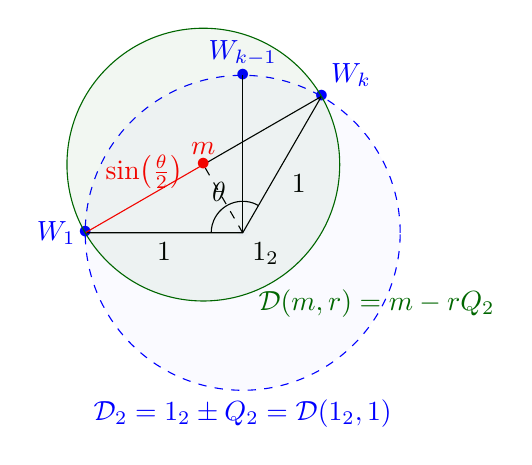
\begin{tikzpicture}
          \draw[dashed,blue,fill, fill opacity = 0.02] (0,0) coordinate (O) node {$\bullet$} circle (2);
          \draw[blue] (0,-2) node[below] {$\mathcal{D}_2 = \mathbbm{1}_2 \pm Q_2 = \mathcal{D}(\mathbbm{1}_2,1)$};
          \draw (O) node[below right] {$\mathbbm{1}_2$};
          \draw[blue] (-2,0) coordinate (A) node {$\bullet$};
          \draw[blue] (A) node[left] {$W_1$};
          \draw[dashed,blue] (0,2) coordinate (B) node {$\bullet$};
          \draw[blue] (B) node[above] {$W_{k-1}$};
          \draw[blue] (1,1.732) coordinate (C) node {$\bullet$};
          \draw[blue] (C) node[above right] {$W_k$};
          \draw (A) -- (O) -- (C);
          \draw (O) -- (B);
          \draw pic["$\theta$", draw=black, angle eccentricity=1.5, angle radius=0.4cm] {angle=C--O--A};
          \coordinate (D) at ($0.5*($(A)+(C)$)$);
          \draw (D) -- (C);
          \draw[dashed] (O) -- (D);
          \draw[red] (A) -- (D);
          \draw[red] ($0.5*($(A)+(D)$)$) node[above] {$\sin(\frac{\theta}{2})$};
          \draw[red] (D) node {$\bullet$};
          \draw[red] (D) node[above] {$m$};
          \draw ($0.5*($(A)+(O)$)$) node[below] {$1$};
          \draw ($0.5*($(C)+(O)$)$) node[below right] {$1$};
          \draw[darkgreen,fill, fill opacity = 0.05] (D) circle (1.732);
          \draw[darkgreen] (1.7,-0.9) node {$\mathcal{D}(m,r) = m - rQ_2$};
        \end{tikzpicture}
      \end{center}
    \end{column}
    \begin{column}{5cm}
      For a set of $k$ pure states:
      \begin{itemize}
        \pause
      \item All of them in one hemisphere: $r =\sin(\frac{\theta}{2})$, so $f_W(S)=1 + \sin(\frac{\theta}{2})$.
        \pause
      \item Otherwise:\\ $r=1$, $f_W(S)=2$.
      \end{itemize}
      \pause
      We recover in particular the example of the beginning.
    \end{column}
  \end{columns}
\end{frame}

%%%%%%%%%%%%%%%%%%%%%%%%%%%%%%%%%%%%%%%%%%
\section{General Convex Problem: MECP}
%%%%%%%%%%%%%%%%%%%%%%%%%%%%%%%%%%%%%%%%%%
%%%%%%%%%%%%%%%%%%%%%%%%%%%%%%%%%%%%%%%%%%
\subsection{MECP general properties}
%%%%%%%%%%%%%%%%%%%%%%%%%%%%%%%%%%%%%%%%%%
\begin{frame}{General Convex Problem}
  For $d > 2$, $\mathcal{D}_d$  not a ball, but still a \emph{convex body}: a full-dimensional compact convex set in $\mathbb{R}^{d^2-1}$

  \pause
  \bigskip
  
  \begin{itemize}
  \item[\underline{MECP:}] \cite{BK13}
    $P \subseteq \mathbb{R}^n$ compact (finite for us), $C \subseteq \mathbb{R}^n$ convex body, find the least dilatation factor $r \geq 0$, such that a translate of $rC$ contains $P$:
    \begin{equation}
      \begin{aligned}
        R(P,C) := && \mini &&& r\\
        && \st &&& P \subseteq m + rC\\
        && &&& m \in \mathbb{R}^n, r \geq 0
      \end{aligned}
    \end{equation}
  \end{itemize}

  
\pause
\bigskip

In particular, MEQP is the case where we take points $P \subseteq \mathcal{D}_d \subseteq \mathbb{R}^{d^2-1}$ and we take $C = -Q_d = \mathbbm{1}_d - \mathcal{D}_d$.\\
In particular $f_W(S) = 1 + R(\set{W_x}_{x \in S},-Q_d)$.
\end{frame}

\begin{frame}{Optimality conditions}
  \begin{columns}
      \begin{column}{7cm}
        \begin{theo}[Optimality conditions]
          \label{optCond}
          $P$ is optimally contained in $C$ iff:
          \begin{enumerate}
          \item $P \subseteq C$
          \item For some $2 \leq k \leq n + 1$, there exist $p_1, \ldots , p_k \in P$ and hyperplanes $H(a_i,1)$ supporting $P$ and $C$ in $p_i$ s.t. $0  \in \text{conv}\set{a_1,\ldots,a_k}$.
          \end{enumerate}
        \end{theo}
      \end{column}

      \begin{column}{5cm}
        \begin{center}
          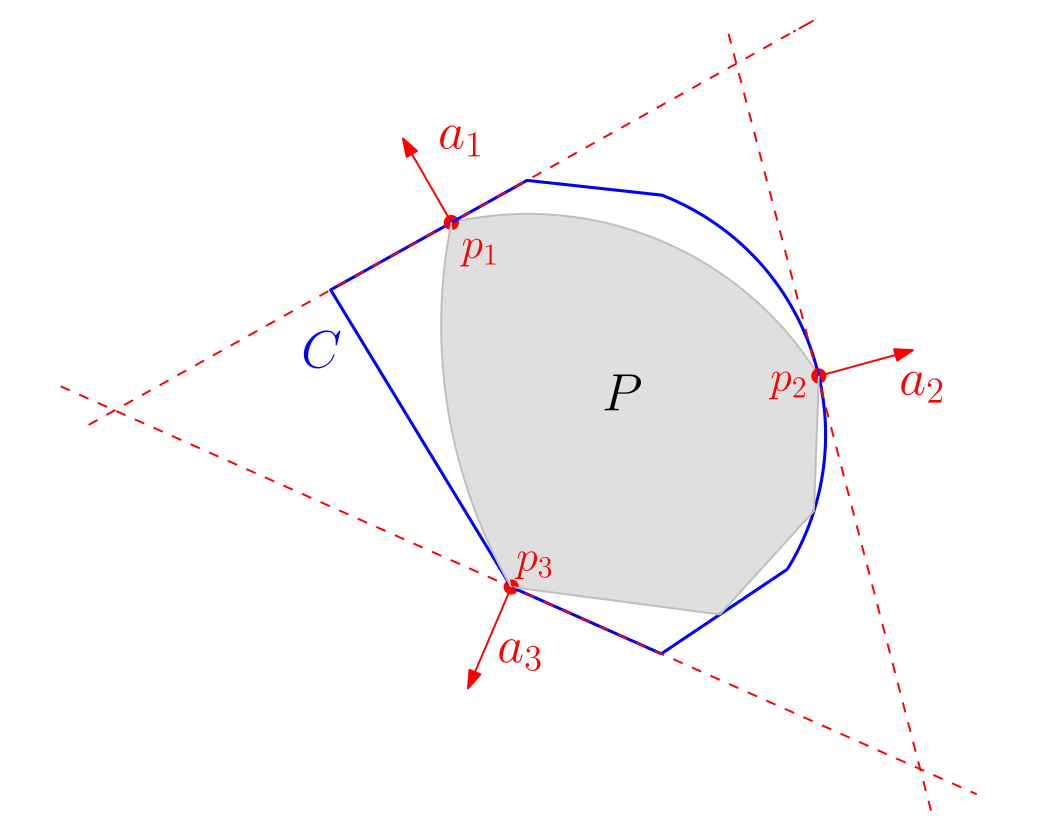
\includegraphics[scale=0.13]{optCond.png}
        \end{center}
      \end{column}
  \end{columns}
\end{frame}

\begin{frame}{Core-radii and $S(W,k)$}
  \begin{defi}[Core-radii]
    The \emph{$k$-th core-radius} of $P$ with respect to $C$ is defined by:
    \[ R_k(P,C) := \underset{S \subseteq P, \abs{S} \leq k+1}{\max} R(S,C) \]
    In particular: $S(W,k) = \frac{1}{k}(1 + R_{k-1}(W,-Q_d))$
  \end{defi}
  \begin{columns}
    \begin{column}{5cm}
      \begin{center}
        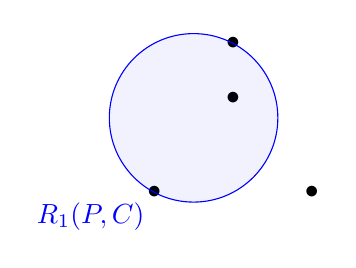
\begin{tikzpicture}
          \draw (0,0) coordinate (A) node {$\bullet$} (2,0) coordinate (B) node {$\bullet$}  (1,1.9) coordinate (C) node {$\bullet$};
          \draw (1,1.2) coordinate (D) node {$\bullet$};
          \draw[darkgreen] ($1/2*($(A)+(C)$)$) coordinate (G);
          \draw[blue,fill,fill opacity=0.05] (G) circle (1.07); 
          \draw[blue] (A) node[below left] {$R_1(P,C)$};
        \end{tikzpicture}
      \end{center}
    \end{column}
    
    \begin{column}{5cm}
      \begin{center}
        \begin{tikzpicture}
          \draw (0,0) coordinate (A) node {$\bullet$} (2,0) coordinate (B) node {$\bullet$} (1,1.9) coordinate (C) node {$\bullet$};
          \draw (1,1.2) coordinate (D) node {$\bullet$};
          \draw[blue,fill,fill opacity=0.05] (G) circle (1.07); 
          \draw[red,fill,fill opacity=0.05] (1,0.69) circle (1.22);
          \draw[red] (B) node[right] {$R_2(P,C)$};
        \end{tikzpicture}
      \end{center}
    \end{column}
  \end{columns}
\end{frame}

\begin{frame}{Properties on core-radii}
  \begin{theo}[Helly's theorem]
    If $\dim(P) \leq k$, then $R_k(P,C) = R(P,C)$. \underline{For us:} $d^2$ measurement outputs used  at most.
  \end{theo}
  
  \pause
  \bigskip
  
  \begin{theo}[$R_k/k$ decreases]
    \[\Big(\frac{R_k(P,C)}{k}\Big)_{k \in [n]} \text{ decreases. \underline{For us:} } \Big(\frac{S(W,k) - \frac{1}{k}}{1 - \frac{1}{k}}\Big)_{k \in [n]} \text{ decreases.}\]
  \end{theo}
\end{frame}

\begin{frame}{$R_k/k$ decreases I}
  \begin{itemize}
  \item Let us show that $\Big(\frac{R_k(P,C)}{k}\Big) \leq \Big(\frac{R_{k-1}(P,C)}{k-1}\Big)$.
    \pause
    \bigskip
  \item $S = \set{x_1, \ldots x_{k+1}} \subseteq P$ s.t. $R(S,C) = R_k(P,C)$: if it does not exist, then $R_k(P,C) = R_{k-1}(P,C)$ and we are done.
  \item We suppose $\sum_{i=1}^{k+1} x_i = 0$ and $R_{k-1}(P,C) = 1$.
    \bigskip
  \item We will show that $R(S,C) \leq \frac{k}{k-1}$.
  \end{itemize}
\end{frame}

\begin{frame}{$R_k/k$ decreases II}
  \begin{columns}
    \begin{column}{5cm}
      \begin{center}
        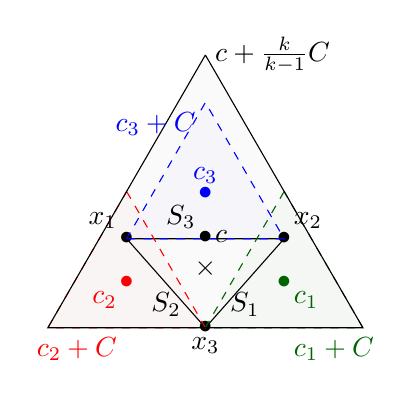
\begin{tikzpicture}
          \draw (0,0) coordinate (A) node {$\bullet$} node[above left] {$x_1$} -- (2,0) coordinate (B) node {$\bullet$}  node[above right] {$x_2$} -- (1,-1.13) coordinate (C) node {$\bullet$}  node[below] {$x_3$} -- (A);
          \draw ($1/2*($(A)+(B)$)$) node[above left] {$S_3$};
          \draw ($1/2*($(A)+(C)$)$) node[below] {$S_2$};
          \draw ($1/2*($(B)+(C)$)$) node[below] {$S_1$};
          \draw[dashed, blue, fill,fill opacity=0.02] (A)--(B)--(1,1.73) coordinate (D)--(A);
          \draw[dashed, red, fill,fill opacity=0.02] ($(A)+(0,0.6)$)--(C)--($(-1,-1.73)+(0,0.6)$) coordinate (E)--($(A)+(0,0.6)$);
          \draw[dashed, darkgreen, fill,fill opacity=0.02] ($(B)+(0,0.6)$)--(C)--($(3,-1.73)+(0,0.6)$) coordinate (F)--($(B)+(0,0.6)$);
          \draw[darkgreen] ($1/3*($($(B)+(0,0.6)$)+(C)+(F)$)$) coordinate (c1) node {$\bullet$} node[below right] {$c_1$};
          \draw[red] ($1/3*($($(A)+(0,0.6)$)
          +(C)+(E)$)$) coordinate (c2) node {$\bullet$} node[below left] {$c_2$};
          \draw[blue] ($1/3*($(A)+(B)+(D)$)$) coordinate (c3)  node {$\bullet$} node[above] {$c_3$};
          \draw ($1/3*($(A)+(B)+(C)$)$) coordinate(0) node {$\times$};
          \draw ($1/3*($(c1)+(c2)+(c3)$)$) coordinate (c0);
          \draw ($(c0)+($($(c0)-(0)$)$)$) coordinate (c) node {$\bullet$} node[right] {$c$};
          \draw ($(c)+(0,2.31)$) coordinate (X) node[right] {$c+\frac{k}{k-1}C$};
          \draw[fill,fill opacity=0.02] (X)--(E)--(F)--(X);
          \draw[darkgreen] ($1/2*($(C)+(F)$)$) node[below right] {$c_1+C$};
          \draw[red] ($1/2*($(C)+(E)$)$) node[below left] {$c_2+C$};
          \draw[blue] (D) node[below left] {$c_3+C$};
        \end{tikzpicture}
      \end{center}
      \end{column}
      
      \begin{column}{7cm}
        \begin{itemize}
        \item $S_j = \text{conv}\set{x_i: i \not= j}$ facets of S.
          \pause          
        \item $-\frac{1}{k}x_j =\frac{1}{k}\sum_{i\not=j}x_j \in S_j$\\
        $x_j \in S_i$ for $i \not= j$
          \pause
          \bigskip
        \item $S_i \subseteq c_i + C$ so $(k-\frac{1}{k})x_j \in \sum_{i=1}^{k+1} S_i \subseteq \sum_{i=1}^{k+1} c_i + (k+1)C$ by convexity of $C$.

          \pause
          \bigskip
        \item Implies $R(S,C) \leq \frac{k+1}{k-\frac{1}{k}}=\frac{k}{k-1}$\\
          with $c = \frac{k}{k-1} \sum_{i=1}^{k+1}\frac{1}{k+1} c_i$ QED.
        \end{itemize}
      \end{column}
  \end{columns}
\end{frame}

\begin{frame}{Greedy algorithm}
      \begin{algorithm}[H]
      \DontPrintSemicolon
      
      \KwInput{$k \in \set{1,\ldots,n}$}
      \KwOutput{An \emph{approximation} of $R_{k-1}(P,C)$: a set $S_k$ of size $k$ such that $R_{k-1}(P,C) \leq (1+c)R(S_k,C)$}
      $S_0 = \emptyset$\\
      \For{$i \in \set{1,\ldots,k}$}
         {
           $p_i = \underset{p \in P-S_{i-1}}{\text{argmax }} R(S_{i-1} \cup \set{p},C)$\\
           $S_i = S_{i-1} \cup \set{p_i}$
         }

         \Return $S_k$
         \caption{Greedy algorithm}
         \label{greedy}
      \end{algorithm}
      
We assume we have an \emph{oracle} that computes $R(S,C)$ for cost $1$. Thus the greedy algorithm is polynomial. Does it give a good approximation ratio $1+c$?
\end{frame}

%%%%%%%%%%%%%%%%%%%%%%%%%%%%%%%%%%%%%%%%%%
\subsection{Particular cases of MECP}
%%%%%%%%%%%%%%%%%%%%%%%%%%%%%%%%%%%%%%%%%%
\begin{frame}{Regular simplex}
  \begin{itemize}
  \item Take points in $T^n$ and $C = -T^n$ where $T^n$ is the $n$-regular simplex centered in $0$. Previous drawing was $T^2$.
  \item Corresponds to the classical case of our channel problem:\\
    $T^n$ is the space of probability distributions of dimension $n+1$.

    \bigskip
    \pause
  \item In \cite{BF17}, it was shown that the greedy algrithm has an approximation ratio $1+c = \frac{1}{1-e^{-1}}$ and that it is optimal if $P \not= NP$.
  \item This was done through the \emph{submodularity} of $f_W$, which is the discrete equivalent of concavity.
  \item However, $f_W$ is not submodular even for one qubit.
      
  \end{itemize}
\end{frame}

\begin{frame}{Ball}
  \begin{itemize}
  \item MECP well studied when $C=\mathbb{B}^n$ is a $n$-ball, known as MEB.
  \item The MEB of $P$ finite can be efficiently approximated (FPTAS).
  \end{itemize}

  \pause
  
  \begin{defi}[Core-set]
    $S \subseteq P$ is a $\epsilon$-\emph{core-set} of P if $R(S,C) \leq R(P,C) \leq (1+\epsilon)R(S,C)$
  \end{defi}

  \begin{theo}[\cite{BK03}]
    \label{coreprop}
    An $\epsilon$-core-set $S_{\epsilon}$ of $P \subseteq \mathbb{R}^n$ of size $\lceil\frac{2}{\epsilon}\rceil$ can be efficiently computed. In particular, this gives a $(1+\frac{2}{k})$-approximation of $R_k(P,C)$.
  \end{theo}

  \pause
  
  \begin{proof}[Proof of Corollary]
    Let $\epsilon$ such that $k+1 = \lceil\frac{2}{\epsilon}\rceil = \abs{S_{\epsilon}}$. Then $\epsilon \leq \frac{2}{k}$, so $R_k(P,C) \leq R(P,C) \leq (1+\epsilon)R(S_{\epsilon},C) \leq (1+\frac{2}{k})R(S_{\epsilon},C)$.
  \end{proof}
\end{frame}

\begin{frame}{Algorithm}
  \begin{algorithm}[H]
      \DontPrintSemicolon
      
      \KwInput{$k \in \set{1, \ldots, n}$}
      \KwOutput{An $\frac{2}{k}$-core-set $S_k$ of $P \subseteq \mathbb{R}^n$ of size $k+1$}
      $S_0 = \set{p}$ with $p$ any point of $P$\\
      $c_0 = p, r_0 = 0$ \tcp*{Center and radius of MEB of $S_0$}
      \For{$i \in \set{1,\ldots,k}$}
         {
           $q_i =$ furthest point from $c_{i-1}$ in $P$\\
           $S_{i} = S_{i-1} \cup \set{q_i}$\\
           $c_i,r_i$ such that MEB($S_i)=\mathcal{B}(c_i,r_i)$\\
         }
         
         \Return $S_k$
         \caption{\cite{BK03} algorithm}
  \end{algorithm}
\end{frame}

\begin{frame}{Example}
  \begin{columns}
    \begin{column}{5cm}
      \begin{center}
        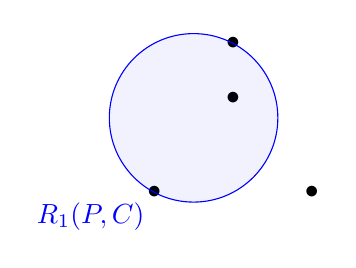
\begin{tikzpicture}
          \draw (0,0) coordinate (A) node {$\bullet$} (2,0) coordinate (B) node {$\bullet$}  (1,1.9) coordinate (C) node {$\bullet$};
          \draw (1,1.2) coordinate (D) node {$\bullet$};
          \draw[darkgreen] ($1/2*($(A)+(C)$)$) coordinate (G);
          \draw[blue,fill,fill opacity=0.05] (G) circle (1.07); 
          \draw[blue] (A) node[below left] {$R_1(P,C)$};
        \end{tikzpicture}
      \end{center}
    \end{column}
    
    \begin{column}{5cm}
      \begin{center}
        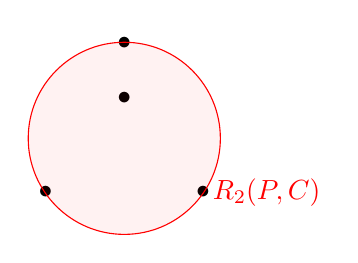
\begin{tikzpicture}
          \draw (0,0) coordinate (A) node {$\bullet$} (2,0) coordinate (B) node {$\bullet$} (1,1.9) coordinate (C) node {$\bullet$};
          \draw (1,1.2) coordinate (D) node {$\bullet$};
          \draw[red,fill,fill opacity=0.05] (1,0.69) circle (1.22);
          \draw[red] (B) node[right] {$R_2(P,C)$};
        \end{tikzpicture}
      \end{center}
    \end{column}
  \end{columns}
  \begin{columns}
    \pause
    \begin{column}{3.5cm}
      \begin{center}
        \begin{tikzpicture}
          \draw (0,0) coordinate (A) node {$\bullet$} node[below left] {$2$} (2,0) coordinate (B) node {$\bullet$}  node[below right] {$3$} (1,1.9) coordinate (C) node {$\bullet$} node[right] {$4$};
          \draw (1,1.2) coordinate (D) node {$\bullet$} node[left] {$1$};
          \draw[blue,fill,fill opacity=0.05] (G) circle (1.07);
          \draw[darkgreen,dashed] (A)--(D)--(C) (D)--(B);
          \draw[darkgreen] ($1/2*($(A)+(D)$)$) coordinate (E) node {$\bullet$} node[right] {$c_1$};
          \draw[darkgreen,fill,fill opacity=0.05] (E) circle (0.79);
          \draw[darkgreen] (-0.6,0.3) node {$S_1$};
        \end{tikzpicture}
      \end{center}
    \end{column}

    \pause
    \begin{column}{3.5cm}
      \begin{center}
        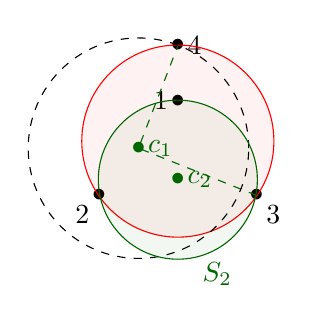
\begin{tikzpicture}
          \draw (0,0) coordinate (A) node {$\bullet$} node[below left] {$2$} (2,0) coordinate (B) node {$\bullet$}  node[below right] {$3$} (1,1.9) coordinate (C) node {$\bullet$} node[right] {$4$};
          \draw (1,1.2) coordinate (D) node {$\bullet$} node[left] {$1$};
          \draw[red,fill,fill opacity=0.05] (1,0.69) circle (1.22);
          \draw[darkgreen] ($1/2*($(A)+(D)$)$) coordinate (E) node {$\bullet$} node[right] {$c_1$};
          \draw[darkgreen,dashed] (B)--(E)--(C);
          \draw[dashed] (E) circle (1.4);
          \draw[darkgreen] (1,0.2) coordinate (F) node {$\bullet$} node[right] {$c_2$};
          \draw[darkgreen,fill,fill opacity=0.05] (F) circle (1.01);      
          \draw[darkgreen] (1.5,-1) node {$S_2$};
        \end{tikzpicture}
      \end{center}
    \end{column}

    \pause
    \begin{column}{4cm}
      \begin{center}
        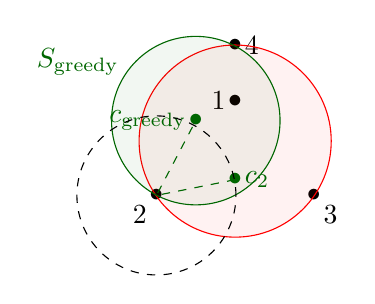
\begin{tikzpicture}
          \draw (0,0) coordinate (A) node {$\bullet$} node[below left] {$2$} (2,0) coordinate (B) node {$\bullet$}  node[below right] {$3$} (1,1.9) coordinate (C) node {$\bullet$} node[right] {$4$};
          \draw (1,1.2) coordinate (D) node {$\bullet$} node[left] {$1$};
          \draw[red,fill,fill opacity=0.05] (1,0.69) circle (1.22);
          \draw[darkgreen] (1,0.2) coordinate (F) node {$\bullet$} node[right] {$c_2$};
          \draw[darkgreen] ($1/2*($(A)+(C)$)$) coordinate (G) node {$\bullet$} node[left] {$c_{\text{greedy}}$};
          \draw[darkgreen,dashed] (F)--(A)--(G);
          \draw[darkgreen,fill,fill opacity=0.05] (G) circle (1.07);
          \draw[darkgreen] (-1,1.7) node {$S_{\text{greedy}}$};
          \draw[dashed] (A) circle (1.01);
        \end{tikzpicture}
      \end{center}
    \end{column}
  \end{columns}
\end{frame}

\begin{frame}{Key lemmas of the proof}
  Theorem on MECP optimality conditions restated for MEB gives:

  \begin{lem}[Half-space lemma]
    $\mathcal{B}(P)$ is the minimum enclosing ball of $P \subseteq \mathbb{R}^n$ iff any closed half-space that contains the center $c_{\mathcal{B}(P)}$ also contains a point of $P$ on the boundary of $\mathcal{B}(P)$.
  \end{lem}

  \pause

\begin{proof}[Proof sketch]
   \begin{itemize}
   \item If $c_{i+1} = c_i$, then we have an MEB of all $P$.
     \pause
   \item Else, take $H \ni c_i$ with $H \perp \overset{\rightarrow}{c_ic}_{i+1}$, and $p \in \partial\mathcal{B}(S_i) \cap H^+ \cap S_i$
  \item Get two inequalities:
    \begin{enumerate}
    \item $r_{i+1} \geq \norm{c_{i+1}-p}_2 \geq \sqrt{r_i^2+\norm{c_{i+1}-c_i}_2^2}$
    \item $r_{i+1} \geq \norm{c_{i+1}-q_{i+1}}_2 \geq R - \norm{c_{i+1}-c_i}_2$
    \end{enumerate}
    \pause
    \item Implies that after $k = \lceil\frac{2}{\epsilon}\rceil$ steps, we get $R \leq (1+\epsilon)r_k$.
  \end{itemize}
 \end{proof}
\end{frame}

\begin{frame}{Optimality of this algorithm}
  \begin{itemize}
  \item The previous algorithm gives a PTAS, ie. for fixed $\epsilon$, we can efficiently compute an $(1+\epsilon)$-approximation of $R_k(P,C)$ for all $k$ and $P$.
    \pause
  \item Indeed, if $\epsilon > \frac{2}{k}$, then $k < \frac{2}{\epsilon}$ is of bounded size: exhaustive search of all sets of size $k$: $\mathcal{O}(\abs{P}^{\frac{2}{\epsilon}})$ efficient for us.
  \item Ohterwise, the previous algorithm works since $\epsilon \leq \frac{2}{k}$.
    \bigskip
    \pause

  \item FPTAS (ie. polynomial in $\frac{1}{\epsilon}$) exists?
  \item No! Reduction form \emph{Exact cover by 3-sets} shows NP-hardness and that no FPTAS exists if $P \not= NP$.
  \end{itemize}
\end{frame}

\begin{frame}{Core-sets in general} 
  \begin{defi}[Core-set]
    $S \subseteq P$ is a $\epsilon$-\emph{core-set} of P if $R(S,C) \leq R(P,C) \leq (1+\epsilon)R(S,C)$\\
    Valid definition in general problem MECP.
  \end{defi}

  \pause
  \bigskip
  
  Not efficient in general:
  \begin{theo}[\cite{BK13}]
    For all $P,C \subseteq \mathbb{R}^n, \epsilon \geq 0$, there exists an $\epsilon$-core-set of size at most $\lceil\frac{n}{1+\epsilon}\rceil+1$.\\
    Moreover, for any $\epsilon < 1$ there exist $P \subseteq \mathbb{R}^n$ and a $0$-symmetric convex body $C$ (ie. $C = -C$) such that no smaller subset of $P$ suffices.\\
    Also, this bound is optimal for the $n$-regular simplex.
  \end{theo}
\end{frame}

\begin{frame}{Quantum states}
  \begin{itemize}
    \item We look at $Q_d = \mathcal{D}_d-\mathbbm{1}_d \subseteq \mathbbm{R}^n$ with $n=d^2-1$.
    \item We have $P \subseteq \mathcal{D}_d = \mathbbm{1}_d + Q_d $ and $C=-Q_d$ in that case.

      \pause
      \bigskip

    \item MEQ of a set of points is unique (counter-example: squares).

      \pause
      
    \item In $C$: $0$ is equidistant from all extremal points (pure states).
    \item $\mathcal{B}\Big(0,\frac{1}{\sqrt{d(d-1)}}\Big) \subseteq C \subseteq \mathcal{B}\Big(0,\sqrt{1-\frac{1}{d}}\Big)$ and tight ratio $d-1$.

      \pause

    \item Like $T^{d-1}$, no $\epsilon$-core-sets of size $< \lceil\frac{d-1}{1+\epsilon}\rceil + 1$:\\
      if $k < \lceil\frac{d-1}{1+\epsilon}\rceil$, then for $\abs{S} \leq k+1$: 
      $R(\mathcal{D}_d,-Q_d)=\frac{d-1}{k}R_k(\mathcal{D}_d,-Q_d) > (1+\epsilon)R_k(\mathcal{D}_d,-Q_d) \geq (1+\epsilon)R(S,-Q_d)$

      \pause
      \bigskip
      
    \item \ldots ?
  \end{itemize}
\end{frame}


%%%%%%%%%%%%%%%%%%%%%%%%%%%%%%%%%%%%%%%%%%
\appendix
%%%%%%%%%%%%%%%%%%%%%%%%%%%%%%%%%%%%%%%%%%
\begin{frame}{Open questions}
  \begin{itemize}
  \item Simplex worst convex shape and ball best convex shape?
    \bigskip
  \item Greedy works well in general (constant approximation ratio)?
    \bigskip
  \item If not in general, what properties do quantum states have that make greedy works?\\
    (experimentally we were unable to find counter-examples)
  \end{itemize}
\end{frame}

\begin{frame}[allowframebreaks]{Bibliographie}
  \bibliographystyle{apalike}
  \bibliography{../These/these.bib}
\end{frame}

%%%%%%%%%%%%%%%%%%%%%%%%%%%%%%%%%%%%%%%%%%
\end{document}
%%%%%%%%%%%%%%%%%%%%%%%%%%%%%%%%%%%%%%%%%%
